%!TeX encoding=utf8
\documentclass[ngerman]{scrartcl} 

\newcommand{\authA}{Daniel Scheiermann}
\newcommand{\matA}{3227680}
\newcommand{\authB}{Felix Springer}
\newcommand{\matB}{10002537}
\newcommand{\grpnr}{SLOT}
\newcommand{\Versuchsnummer}{IQ18}
\newcommand{\Versuchsname}{Scanning Laser Optical Tomography}


%%%%%%%%%%%%%%%%%%Capitalized Color - start%%%%%%%%%%%%%%%%%%%%%%%%
\usepackage{xparse}
\usepackage{xcolor}


\ExplSyntaxOn
\NewDocumentCommand{\colorcap}{ O{blue} m }
 {
  \sheljohn_colorcap:nn { #1 } { #2 }
 }

\tl_new:N \l__sheljohn_colorcap_input_tl
\cs_new_protected:Npn \sheljohn_colorcap:nn #1 #2
 {
  % store the string in a variable for usage with \regex_replace_all:nnN
  \tl_set:Nn \l__sheljohn_colorcap_input_tl { #2 }
  \regex_replace_all:nnN
   { ([A-Z]+) } % search a capital letter (or more)
   { \c{textcolor}\cB\{#1\cE\}\cB\{\1\cE\} } % replace the match with \textcolor{#1}{<match>}
   \l__sheljohn_colorcap_input_tl
  \tl_use:N \l__sheljohn_colorcap_input_tl
 }
\ExplSyntaxOff
%%%%%%%%%%%%%%%%%%Capitalized Color - end%%%%%%%%%%%%%%%%%%%%%%%%
%---configure pagelayout
\KOMAoptions{ % read documentation for KOMAScript providing the documentclass scrartcl
DIV=11,
BCOR=0mm,
paper=a4,
fontsize=12pt,
parskip=half,
twoside=false,
titlepage=true
}

%\usepackage[ %Set linespacing
%singlespacing %onehalfspacing,doublespacing
%]{setspace} 

\usepackage[headsepline,footsepline,automark,pagestyleset=KOMA-Script,markcase=ignoreuppercase]{scrlayer-scrpage} %Configure headline and footer

\clearscrheadings
\setlength{\headheight}{3.5\baselineskip}

\ihead[]{\authB~(\matB)\\\authA~(\matA)}
\ohead{
\includegraphics[height=13pt]{IMAGE/luh_logo.png} \\ \Versuchsnummer $ $ \grpnr}

\cfoot{\vspace{-0.75cm}\pagemark}
\pagestyle{scrheadings}

%better positioning of floatings
\renewcommand{\floatpagefraction}{.75} % standard: .5
\renewcommand{\textfraction}{.1} % standard: .2
\renewcommand{\topfraction}{.8} % standard: .7
\renewcommand{\bottomfraction}{.5} % standard: .3
\setcounter{topnumber}{3} % standard: 2
\setcounter{bottomnumber}{2} % standard: 1
\setcounter{totalnumber}{5} % standard: 3

%---Language and umlauts
\usepackage[utf8]{inputenc} %Set UTF-8 encoding, enables ä,ö,ü etc.
\usepackage[ngerman]{babel} %Set document language to ngerman (new german)  
%\usepackage[% improved hyphenation
%expansion=true,
%protrusion=true
%]{microtype}
\usepackage{subcaption}
%\usepackage{subfig} %subcaption includes subfig
%\captionsetup[subfigure]{list=true, font=large, labelfont=bf, 
%labelformat=brace, position=top}

%---Mathmatics (AMS packages )
\usepackage{amsmath} %generell math enviorments e.g. align
\usepackage{amsfonts}
\usepackage{amssymb} 
%\usepackage{amsthm} %math theorems
%\usepackage{upgreek}%provide special form of greek letters e.g. \upmu
\usepackage{float}
%---Units
\usepackage[decimalsymbol=comma]{siunitx}
%\usepackage{units}
%\usepackage[numbers]{natbib}
%\usepackage{pdfpages}
\usepackage{textcomp}
\usepackage{longtable}
%\usepackage{braket}
%\usepackage{color}

%\renewcommand{\arraystretch}{1.2} % Standard-Zeilenhöhe einstellen

%---tables and imgaes
\usepackage{graphicx} %provide \includegraphics[options]{name}
%\usepackage{epstopdf} %enable the use of eps-graphics
\usepackage[hypcap]{caption} %captions out of floating-enviorments(figure,table)
\usepackage{booktabs} %extra lines in tabulars
%\usepackage{flafter} %Place floating-enviorments after references.
%\usepackage[ %
%section %latest ancor for floating-enviorments
%]{placeins}
%\usepackage{verbatim} %long comments \begin{comment} ...\end{comment}

%---Hyperlinks
\usepackage{hyperref} %create table of content and references as links
\hypersetup{
%
%Colors 
colorlinks=true, 
breaklinks=true, 
citecolor=blue, 
linkcolor=black, 
menucolor=red, 
urlcolor=cyan,
%
%pdf-bookmarks
bookmarksopen=false, 
bookmarksopenlevel=0,
% 
%pdf-data
% pdftitle={\titel}, 
% pdfauthor={\writer}, 
% pdfcreator={\writer}, 
% pdfsubject={\titel}, 
% pdfkeywords={\titel} 
%
%misc
plainpages=false,% zur korrekten Erstellung der Bookmarks 
hypertexnames=false,% zur korrekten Erstellung der Bookmarks 
% hyperindex=true,
}


\begin{document}
\title{\Versuchsname $ $ \Versuchsnummer}
\subtitle{Laborpraktikum durchgeführt im Block 1\\
22.10.2018 – 09.11.2018\vspace{1cm}\\ 
\includegraphics[width=.75\linewidth]{IMAGE/luh_logo.png}}
\author{
\authA\\
\matA
\and
\authB\\
\matB
}
\date{\today}

\pagestyle{empty} %Clear headline and footer
\setcounter{page}{0} %Set pagenumber to 0
\maketitle %Create the title

\newpage 

\thispagestyle{empty}
\tableofcontents
\pagestyle{scrheadings}

\setcounter{page}{1}
\newpage


\section{Einleitung}
In diesem Versuch wird die Methode der Tomographie am Beispiel der SLOT \\ \glqq \colorcap[luh_blue]{Scanning Laser Optical Tomography}\grqq{} untersucht. Dieses ist ein spezielles dreidimensionales Tomographie-Verfahren, das mit Lasern verschiedener Wellenlängen  Streuung, Absorption und Fluoreszenz als Kontrastmechanismen nutzt.\\

Das dreidimensionale Präparat wird ebenenweise durch zweidimensionale Schnitte (Tomogramme) rekonstruiert und zu einem dreidimensionalen Bildobjekt zusammengesetzt. Das entstandene Bildobjekt ist nun vom Präparat getrennt und virtuell verfügbar. Daraus ergibt sich der Vorteil das Präparat unbeschädigt lassen zu können und dennoch die innere Struktur des Präparates zu untersuchen \cite{Anleitung}.\\

\section{Scanning Laser Optical Tomography}

\subsection{Radontransformation}
Bei allen auf Computertomographie basierenden Verfahren ist die Radontransformation die mathematische Grundlage zur Nutzung des integrierten Signals für eine 3D-Darstellung.
Beim Durchleuchten des Präparats führt jegliche Wechselwirkung mit dem Präparat zu einer veränderten Intensität des eingestrahlten Lichtes.
Nimmt man hinter dem Präparat dieses Signal für eine festen Einstrahlungswinkel $\phi$ auf, so erhält man eine über die Lauflinie des Strahls integrierte Signalabschwächung.
Diese bildet einen Funktionswert der Radontransformierten $R(\rho,\phi)$ zu einem festen $\phi$.
Durch Abrastern entlang des Präparats, also Variation von $\rho$, erhält dann die gesamte Radontransformierte die in direktem Verhältnis zum Tomogramm der gescannten Ebene des Präparats steht.
Scannt man das Präparat zusätzlich in $z$-Richtung, so erhält man Tomogramme, die zusammengenommen zu einem Tomographen und damit zu einem 3D-Objekt zusammengeführt werden können, das auch Informationen über das Innere des Präparats preisgibt.

%DONE: \textcolor{red}{Letzter Satz nicht falsch aber ausführlicher.}

Die Strahlen werden hierfür in Polarkoordinaten durch eine Schar von Geraden parametrisiert. Durch den Polarwinkel $\phi$ ist die Richtung der Strahlen und durch $s$ wird der \glqq Radius\grqq{} festgelegt. Weiterhin wird durch $\rho$ der senkrechte Abstand von der Geraden, die im Winkel $\phi$ durch den Ursprung geht, festgelegt, wodurch die Schar der Strahlen parametrisiert wird.  
\begin{equation}
lin_{\rho,\phi}(s) = \begin{pmatrix}
\cos(\phi) & -\sin(\phi)  \\
\sin(\phi) & \cos(\phi) \\
\end{pmatrix}
\cdot
\begin{pmatrix}
\rho \\
s \\
\end{pmatrix}
 =
\begin{pmatrix}
\rho \cdot \cos(\phi) - s \cdot \sin(\phi) \\
\rho \cdot \sin(\phi) + s \cdot \cos(\phi) \\
\end{pmatrix}
\end{equation}

%\begin{minipage}{\linewidth}
\begin{figure}
	\centering
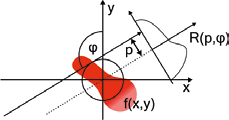
\includegraphics[width=0.6\linewidth]{IMAGE/radon.png}
	\caption{Graphische Darstellung der Radontransformation: Parametrisierung eines Strahls $lin_{\rho,\phi}(s)$ in Polarkoordinaten, wobei $s$ dem Radius und $\phi$ der Polarwinkel ist. Die Schar an Strahlen wird durch $\rho$ parametrisiert.
Das Präparat wird durch die rote Fläche $f(x,y)$ dargestellt und hinter dem Präparat ist das integrierte Signal über die verschiedenen Strahlen der Schar dargestellt, die zusammengenommen die Radontransformierte $R(\rho, \phi)$ ergeben \cite{slot_paper}.}
	\label{fig:radon}
\end{figure}

Für eine zweidimensionale Funktion $f(x,y)$ ist die Radontransformierte das integrierte Signal über den parametrisierten Weg durch das Präparat:

\begin{equation}
R(\rho,\phi) = \int_{- \infty}^{\infty} f(lin_{p,q}(s)) \,\mathrm{d}s
=
\int_{- \infty}^{\infty} f\begin{pmatrix}
\rho \cdot \cos(\phi) - s \cdot \sin(\phi) \\
\rho \cdot \sin(\phi) + s \cdot \cos(\phi) \\
\end{pmatrix} \,\mathrm{d}s
\end{equation}

Entscheidend für die Nutzung der Tomographie ist die Invertierbarkeit der Radontransformierten $R(\rho,\phi)$, denn dies ermöglicht die Rekonstruktion der ursprünglichen Funktion $f(x,y)$, also die Rekonstruktion des Präparates \cite{slot_paper}.
%\end{minipage}

\subsection{Funktionsweise}
%\begin{minipage}{\linewidth}
Die Funktionsweise von SLOT wird anhand des Schemas in Abbildung \ref{fig:schema} beschrieben.
SLOT basiert auf einem x-y-Scanner-System mit zwei Silberspiegeln, das den auf die Mitte des Präparates fokussierten Laser ablenkt und somit die Probe abrastert.
Das Präparat muss optisch transparent sein, um Streuung innerhalb des Präparats zu verringern und eine höhere Transmission zu erreichen.
Hierzu werden Glycerin oder ähnliche Lösungsmittel genutzt, da diese einen ähnlichen Brechungsindex wie feste organische Bestandteile haben.
Das transmittierte Laserlicht wird von einer Photodiode hinter der Probenkammer detektiert.
Um eine Rekonstruktion durchführen zu können sind Aufnahmen des Präparats von verschiedenen Richtungen nötig.
Diese verschiedenen Aufnahmen werden durch einen Motor ermöglicht, der die Kapillare und damit das Präparat dreht.
Weiterhin regt das Laserlicht das Präparat zur Fluoreszenz an.
Dieses Fluoreszenzlicht wird mittels plankovexen Linsen mit dazwischen liegendem Fluoreszenz-Filter gesammelt und auf den sensitiven Photomuliplier (PMT) geleitet \cite{Anleitung}.\\

\begin{figure}
	\centering
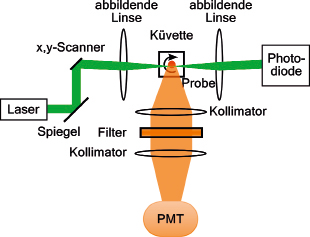
\includegraphics[width=0.8\linewidth]{IMAGE/slot_schema.png}
	\caption{Schema eines scannenden laseroptischen Tomographen (SLOT) \cite{slot_paper}. 
	Der schematische Kollimator ist im Versuchsaufbau ein Bündel von Glasfasern, das an die Unterseite der Küvette angebracht ist und mit der Form eine ähnliche Fläche ausfüllt wie die Photomultiplier-Diode (PMT), sodass möglichst viel der Diode ausgeleuchtet werden kann.
	Der Nutzen des Kollimator ist das gesammelte Licht senkrecht auf die dieelektrischen Farbfilter zu leiten, denn nur dann sind die angegebenen Werte des Herstellers bezüglich der Transmission bestimmter Wellenlängen verlässlich. Ansonsten treten Abweichung der Reflexion und Transmission in Abhängigkeit vom Einfallswinkel entsprechend den Fresnelschen Formeln auf.}
	%DONE: \textcolor{red}{Ausführlicher, insbesondere soll die Abbildung für vollständig aus der Bildunterschrift erklärbar sein.
%Der schematische Kollimator ist im Versuchsaufbau ein Bündel von Glasfasern, das an die Unterseite der Küvette angebracht ist und mit der Form eine ähnliche Fläche ausfüllt wie die PMT-Diode, sodass möglichst viel der Diode ausgeluchtet werden kann.
%Der Kollimator wird genutzt, um das gesammelte Licht senkrecht auf die dieelektrischen Farbfilter zu leiten, denn nur dann sind die angegebenen Werte des Herstellers verlässlich (sonstige Abweichung der Reflexion und Transmission in Abhängigkeit vom Einfallswinkel nach Fresnel-Gesetz}}
	\label{fig:schema}
\end{figure} 
%\end{minipage}

%%%nopagebreak (gehört zusammen)
% \nopagebreak
% \hrule height 0pt
% \pagebreak[2]
%%% 

\subsection{Versuchsaufbau}

%\begin{minipage}{\linewidth}
\begin{figure}[H]
	\centering
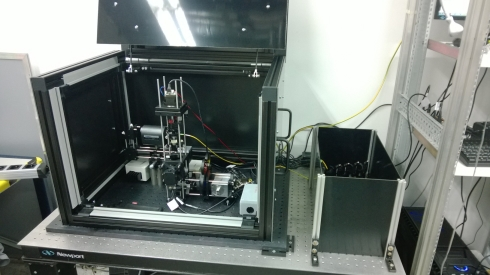
\includegraphics[width=1.0\linewidth]{IMAGE/versuchsaufbau.png}
	\caption{Versuchsaufbau: Der gesamte Versuchsaufbau befindet sich auf einer optischen Platte, um Störungen durch Vibration zu verringern. Weiterhin ist die Kompaktheit des Versuchsaufbaus zu sehen \cite{Anleitung}.}
	\label{fig:versuchsaufbau}
\end{figure} 

\begin{figure}[H]
	\centering
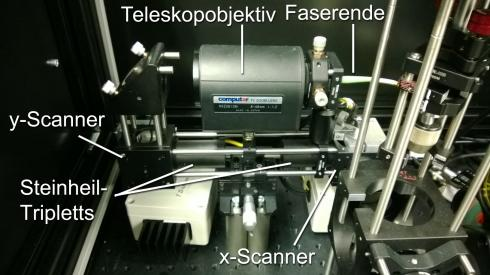
\includegraphics[width=1.0\linewidth]{IMAGE/scanner.jpeg}
	\caption{Das Teleskop ist für die Fokussierung und ermöglicht eine gewisse Flexibilität bei der Einstellung des Strahlendurchmessers des scannenden Lichtstrahls. Weiterhin sind x- und y-Scanner, die das Abrastern des Präparats ermöglichen, zusehen. \cite{Anleitung}. \textcolor{red}{Steinheil-Tripletts}}
	\label{fig:scanner}
\end{figure}

%\end{minipage}



\begin{figure}
\begin{subfigure}[b]{0.5\linewidth}
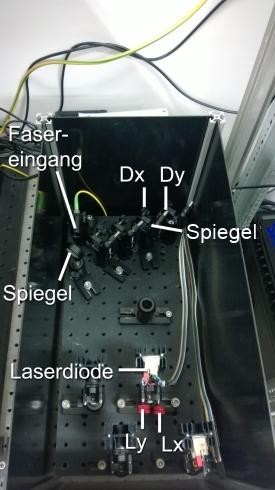
\includegraphics[width=0.98\linewidth]{IMAGE/einkopplung.jpeg}
\label{fig:einkopplung}
	\subcaption{Die Ausrichtung der Laserdioden und der Spiegel in x- und y-Richtung ermöglicht mittels \glqq Beam-Walk \grqq{} die Einkopplung des Lichts zweier Laserdioden mit den Wellenlängen $\lambda = 450 \, nm$ \\  und $\lambda = 520 \, nm$.}
	
	%DONE: \textcolor{red}{Ausführlicher}}
\end{subfigure}
\begin{subfigure}[b]{0.5\linewidth}
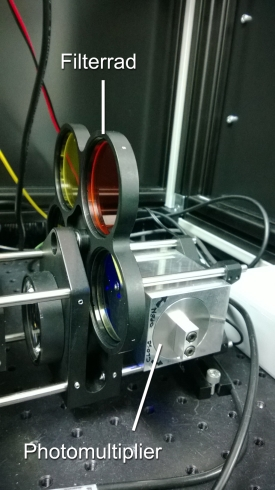
\includegraphics[width=0.98\linewidth]{IMAGE/pmt.png}\label{fig:pmt}
	\subcaption[c]{Das Filterrad wird zur Selektion des Wellenbereichs genutzt, der detektiert werden soll und der Photomuliplier (PMT) wird genutzt, um das wenige Fluoreszenzlicht zu detektieren und für die Tomographie nutzbar zu machen.}
	%DONE: \textcolor{red}{Ausführlicher}}
\end{subfigure}

\caption{Trennung der Laserkonfiguration vom restlichen Versuchsaufbau zur Verringerung der Wahrscheinlichkeit die Ergebnisse der Einkopplung des Diodenlichtes beim Experementieren zu nichte zu machen. \cite{Anleitung}.
	Weiterhin werden Dichromaten genutzt, um durch die selben Reflexionsobjekte verschiedene Wellenlängen einkoppeln zu können und das Experimentieren mit unterschiedlichen Wellenlängen durch An- und Ausschalten der entsprechenden Laserdioden problemlos gelingt. \\}
%DONE: \textcolor{red}{Ausführlicher}}
\end{figure}
%%%%%%%%%%%%%%%
\clearpage

\begin{minipage}{\linewidth}
\begin{figure}[H]
	\centering
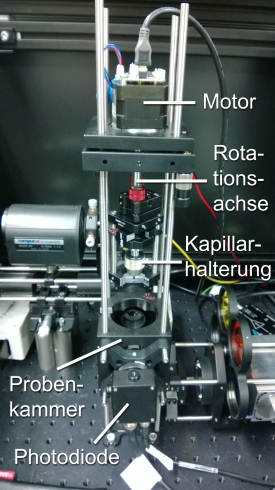
\includegraphics[width=0.491\linewidth]{IMAGE/turm.png}
	\caption{Zusehen ist der Turm mit der Rotationsachse, die beim Versuch dann mittels Kapillarhalterung das in einer Kapillare fixierte Präparat rotiert.
In der Probenkammer wird dann eine Küvette mit Glycerin aus oben genannten Gründen stehen, in die die Kapillare eingetaucht ist. \cite{Anleitung}.
	%DONE: \textcolor{red}{Ausführlicher}
	}
	\label{fig:turm}
\end{figure}

\section{Ergebnisse}
\subsection{Auflösungsvermögen}
Der Kontrast wurde für verschiedene Fokussierungen, Strahlendurchmesser und Wellenlängen des Lasers mithilfe eines USAF-Targets gemessen. Dadurch ergibt sich die Modulationsübertragungsfunktion.\\ 
 \textcolor{red}{Nicht Auflösung sondern lp/mm.}
Bei allen Messungen wurde die Dunkelaufnahme von der Abbildung des Targets abgezogen, um ein Rauschen herauszurechnen.\\
Für geringe Auflösung wurde die Modulationsübertragungsfunktion  in Abhängikeit zur horizontalen Auflösung in Abbildung \ref{fig:Versuch2_Plot2h1} und zur vertikalen Auflösung in Abbildung \ref{fig:Versuch2_Plot2v1} dargestellt.\\
\end{minipage}

\begin{minipage}{\linewidth}
\begin{figure}[H]
	\centering
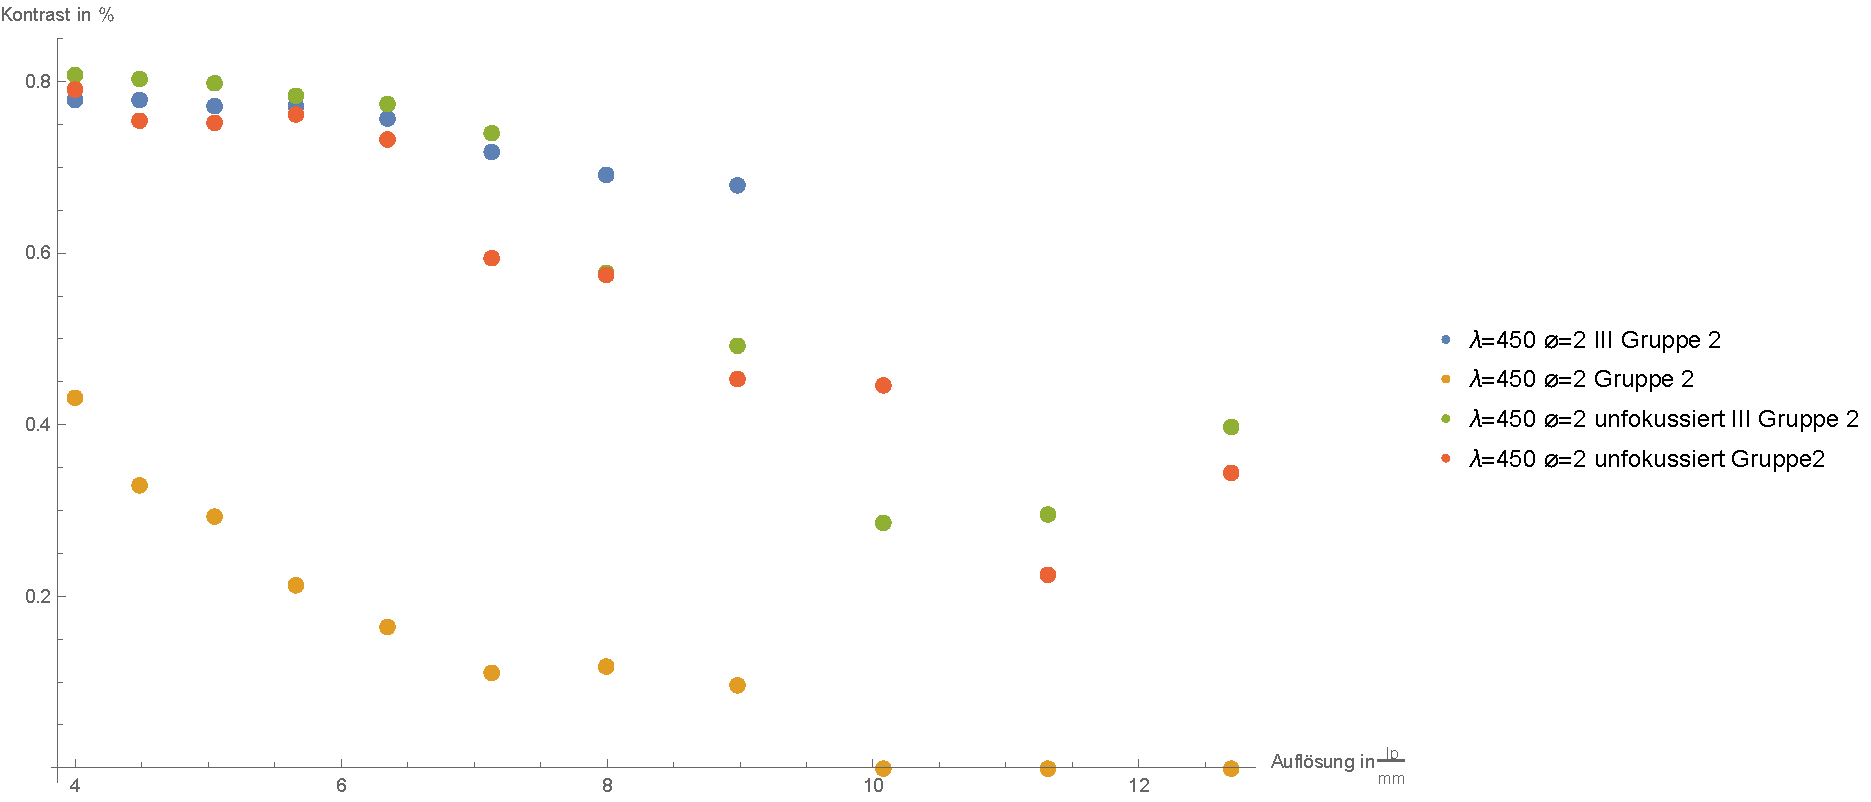
\includegraphics[width=1.0\linewidth]{IMAGE/Versuch2Plot1horizontal2.pdf}
	\caption{Kontrast bei geringer Auflösung (horizontal) \textcolor{red}{Ausführlicher. Was ist III?}}
	\label{fig:Versuch2_Plot2h1}
\end{figure} 

\begin{figure}[H]
	\centering
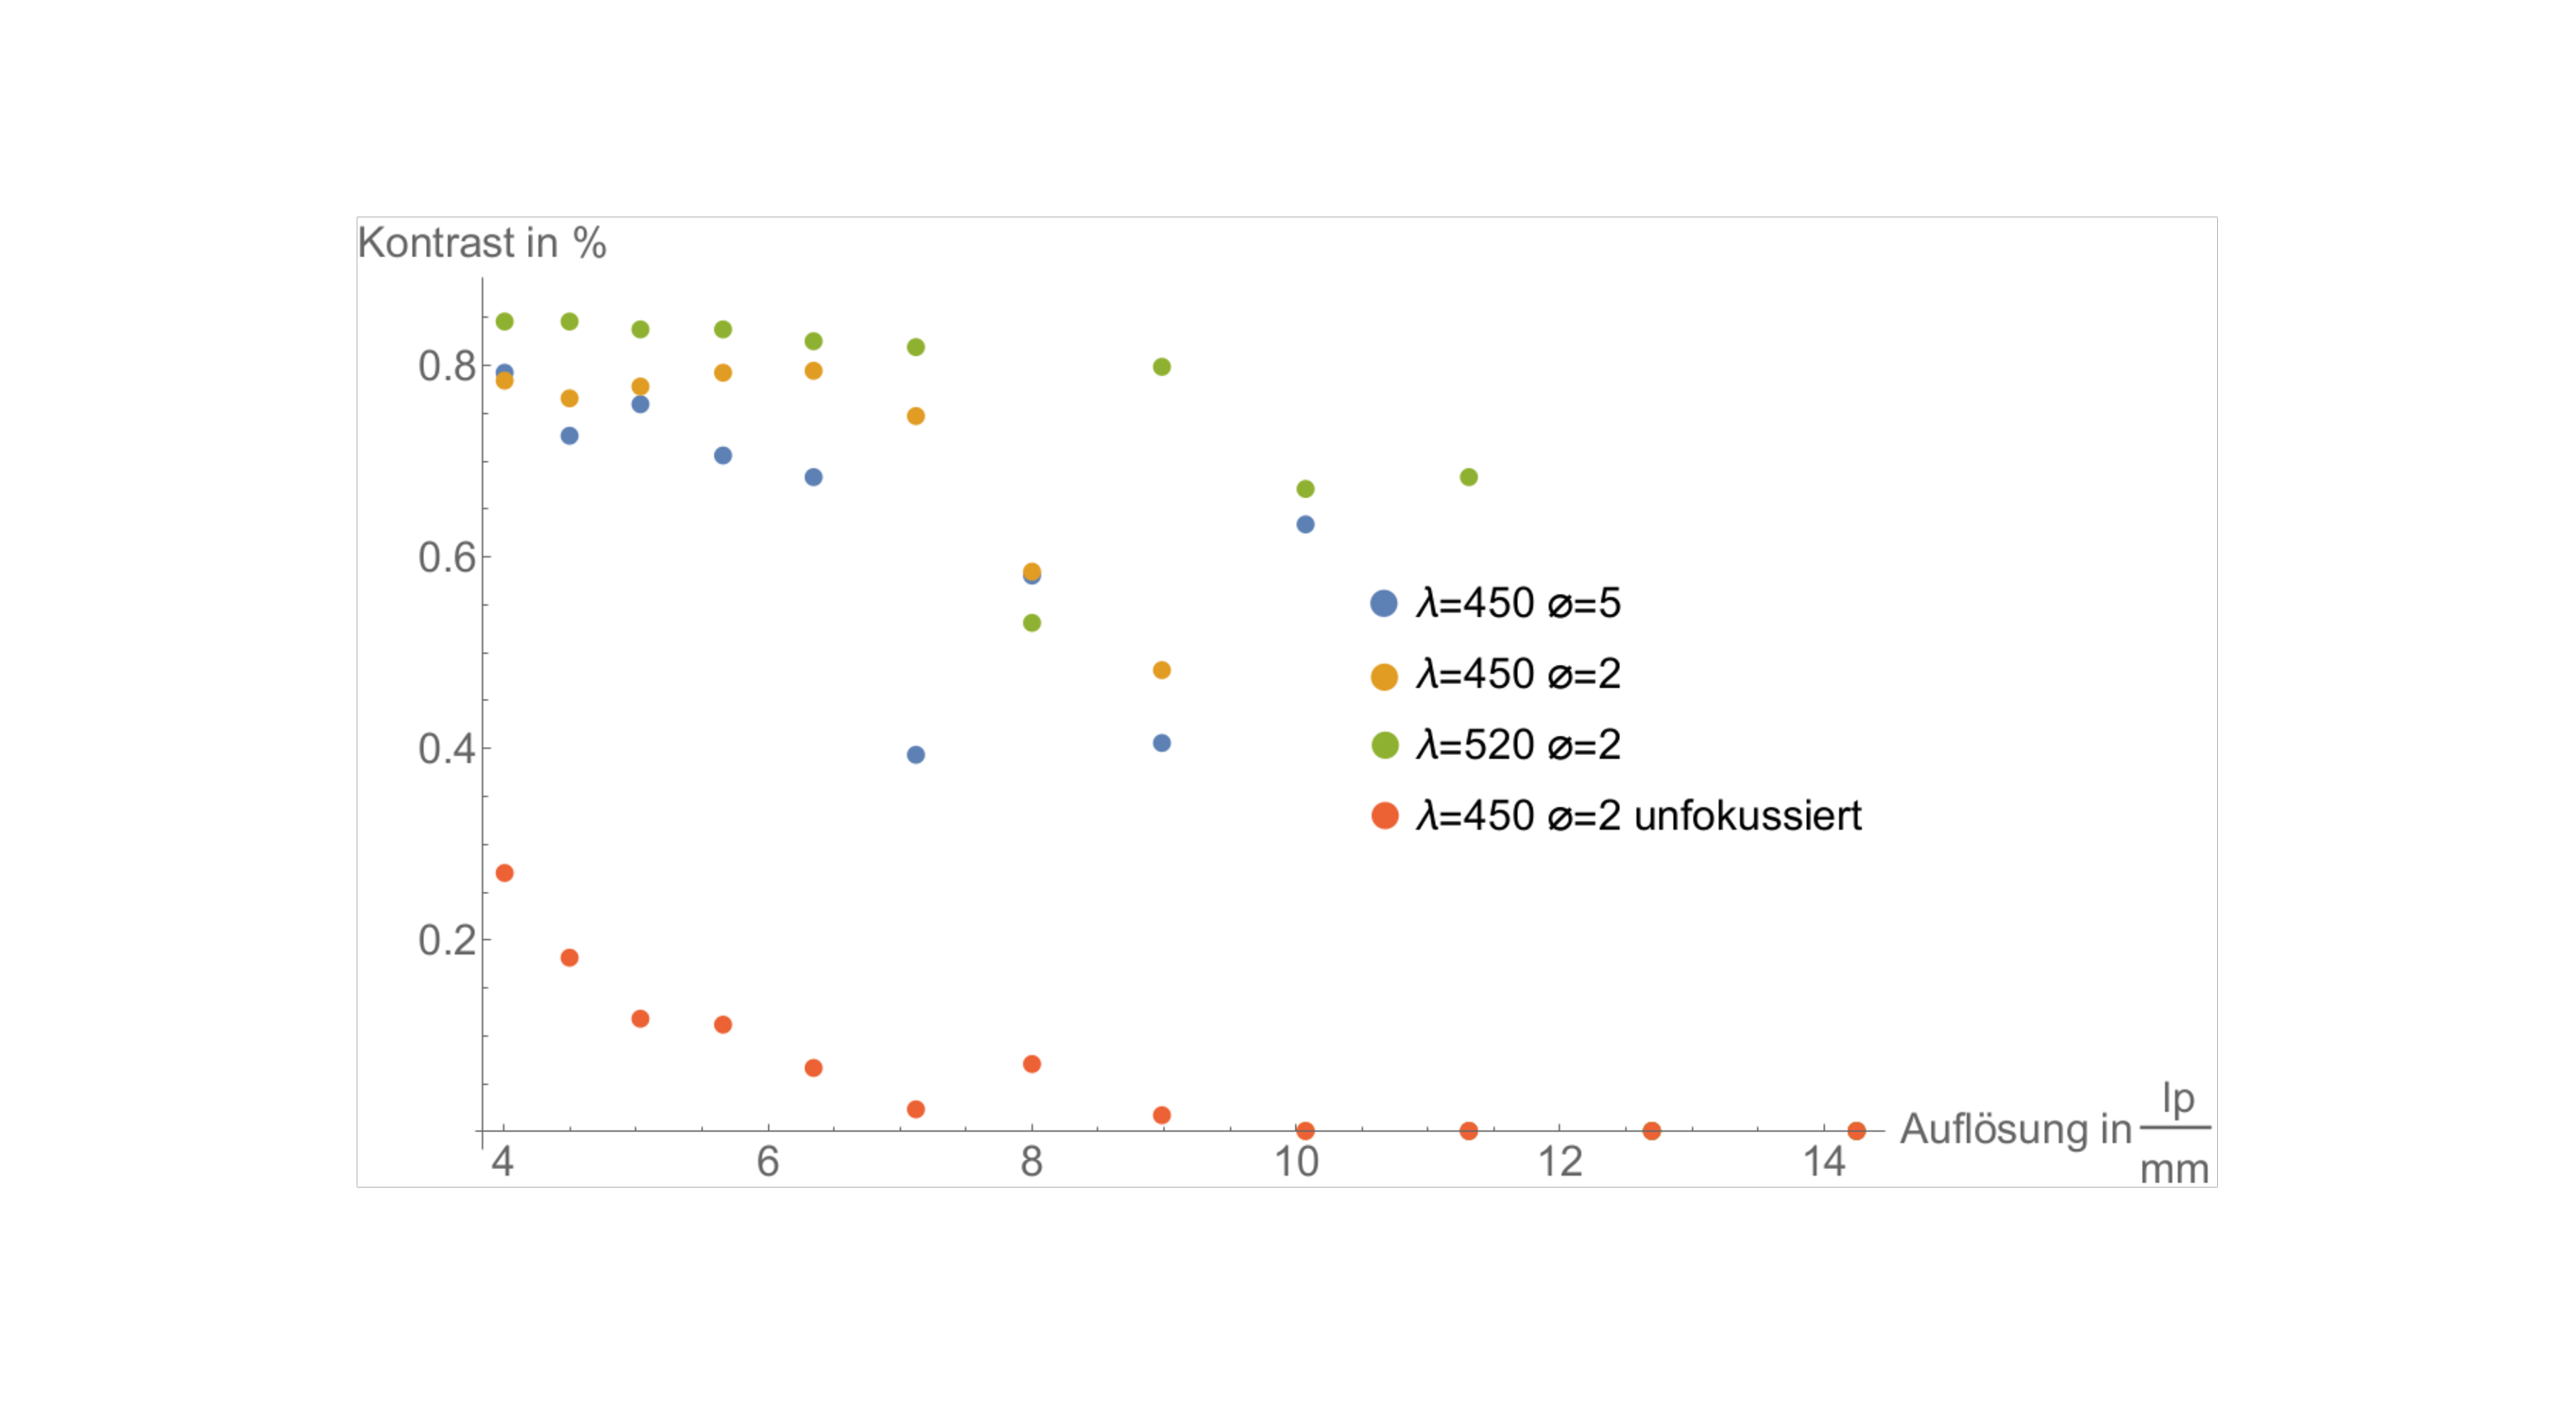
\includegraphics[width=1.0\linewidth]{IMAGE/Versuch2Plot1vertikal2.pdf}
	\caption{Kontrast bei geringer Auflösung (vertikal)}
	\label{fig:Versuch2_Plot2v1}
\end{figure} 

\end{minipage}

\begin{minipage}{\linewidth}
Ein erhöhter Strahlendurchmesser verbessert den Kontrast.\\
Bei geringer Auflösung ist der Kontrast für eine höhere Wellenlänge höher.\\
Der Kontrast ist in horizontaler und vertikaler Richtung von vergleichbarer Höhe.\\
Weiterhin sinkt der Kontrast rapide, falls ohne Fokussierung gemessen wird.

Für hohe Auflösung ist diese zur horizontalen Auflösung in Abbildung \ref{fig:Versuch2_Plot2h2} und zur vertikalen Auflösung in Abbildung \ref{fig:Versuch2_Plot2v2} dargestellt.
\begin{figure}[H]
	\centering
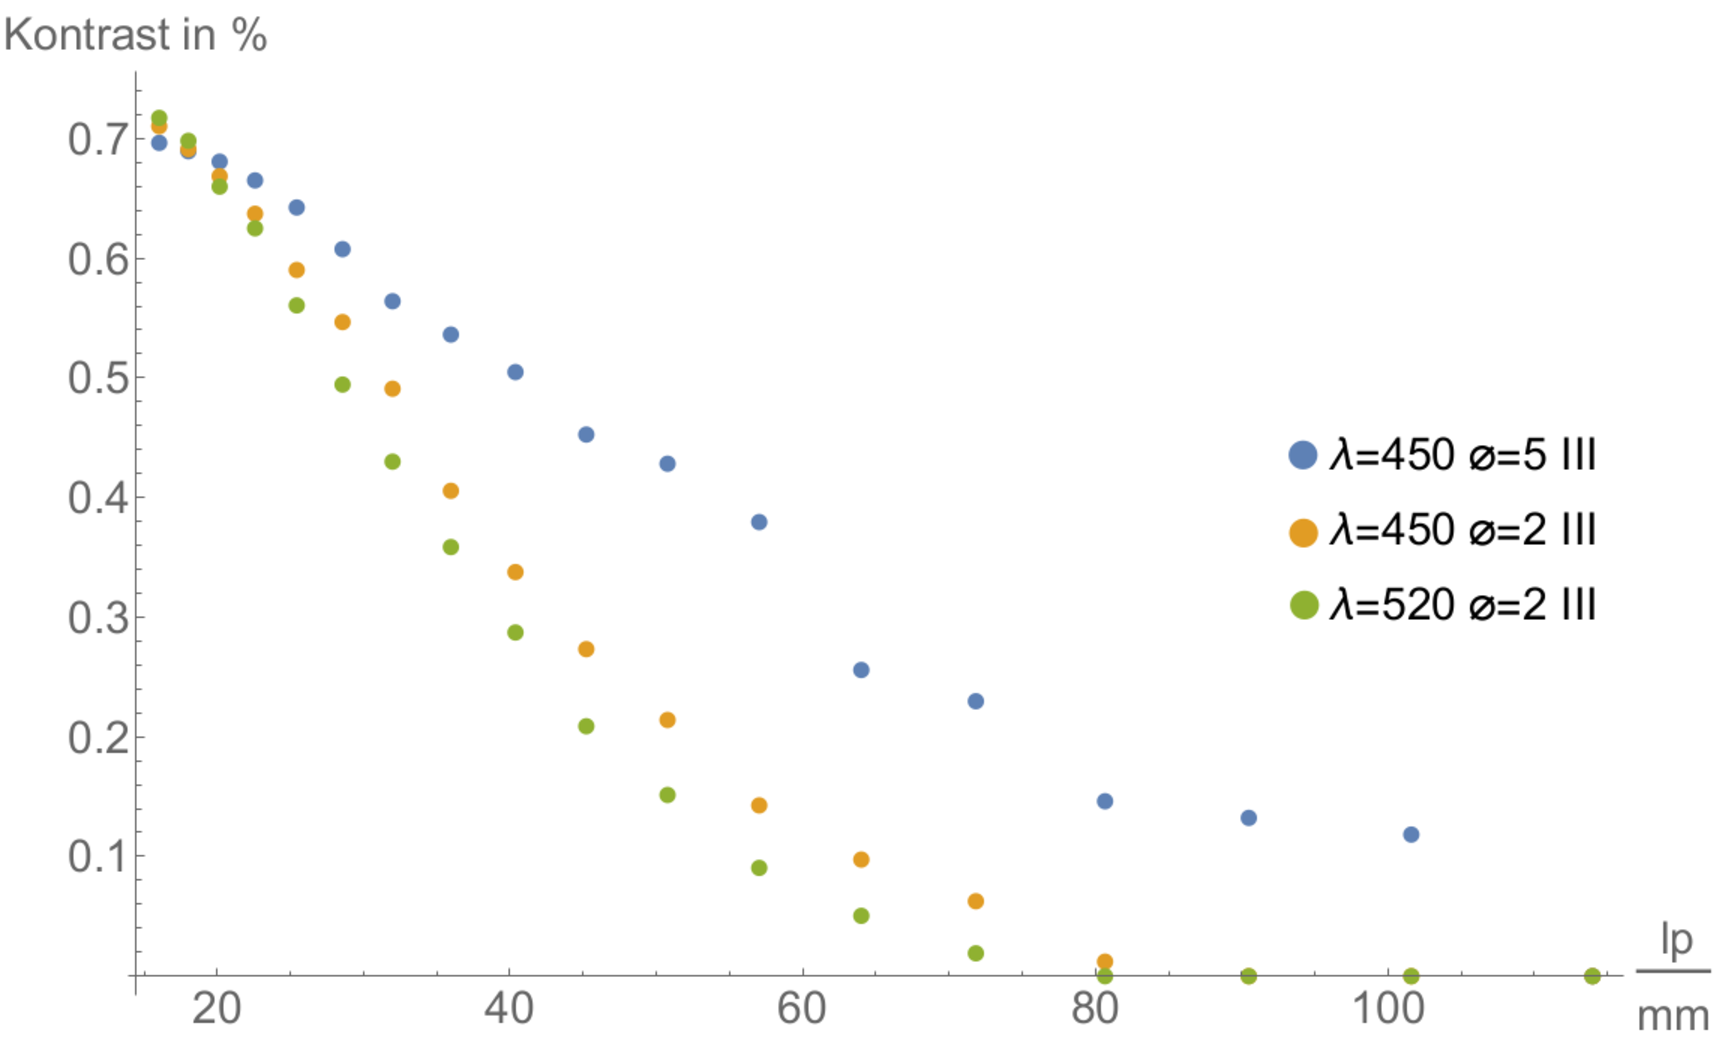
\includegraphics[width=1.0\linewidth]{IMAGE/Versuch2Plot2horizontal2.pdf}
	\caption{Kontrast bei hoher Auflösung (horizontal)}
	\label{fig:Versuch2_Plot2h2}
\end{figure} 
\end{minipage}

\begin{figure}[H]
	\centering
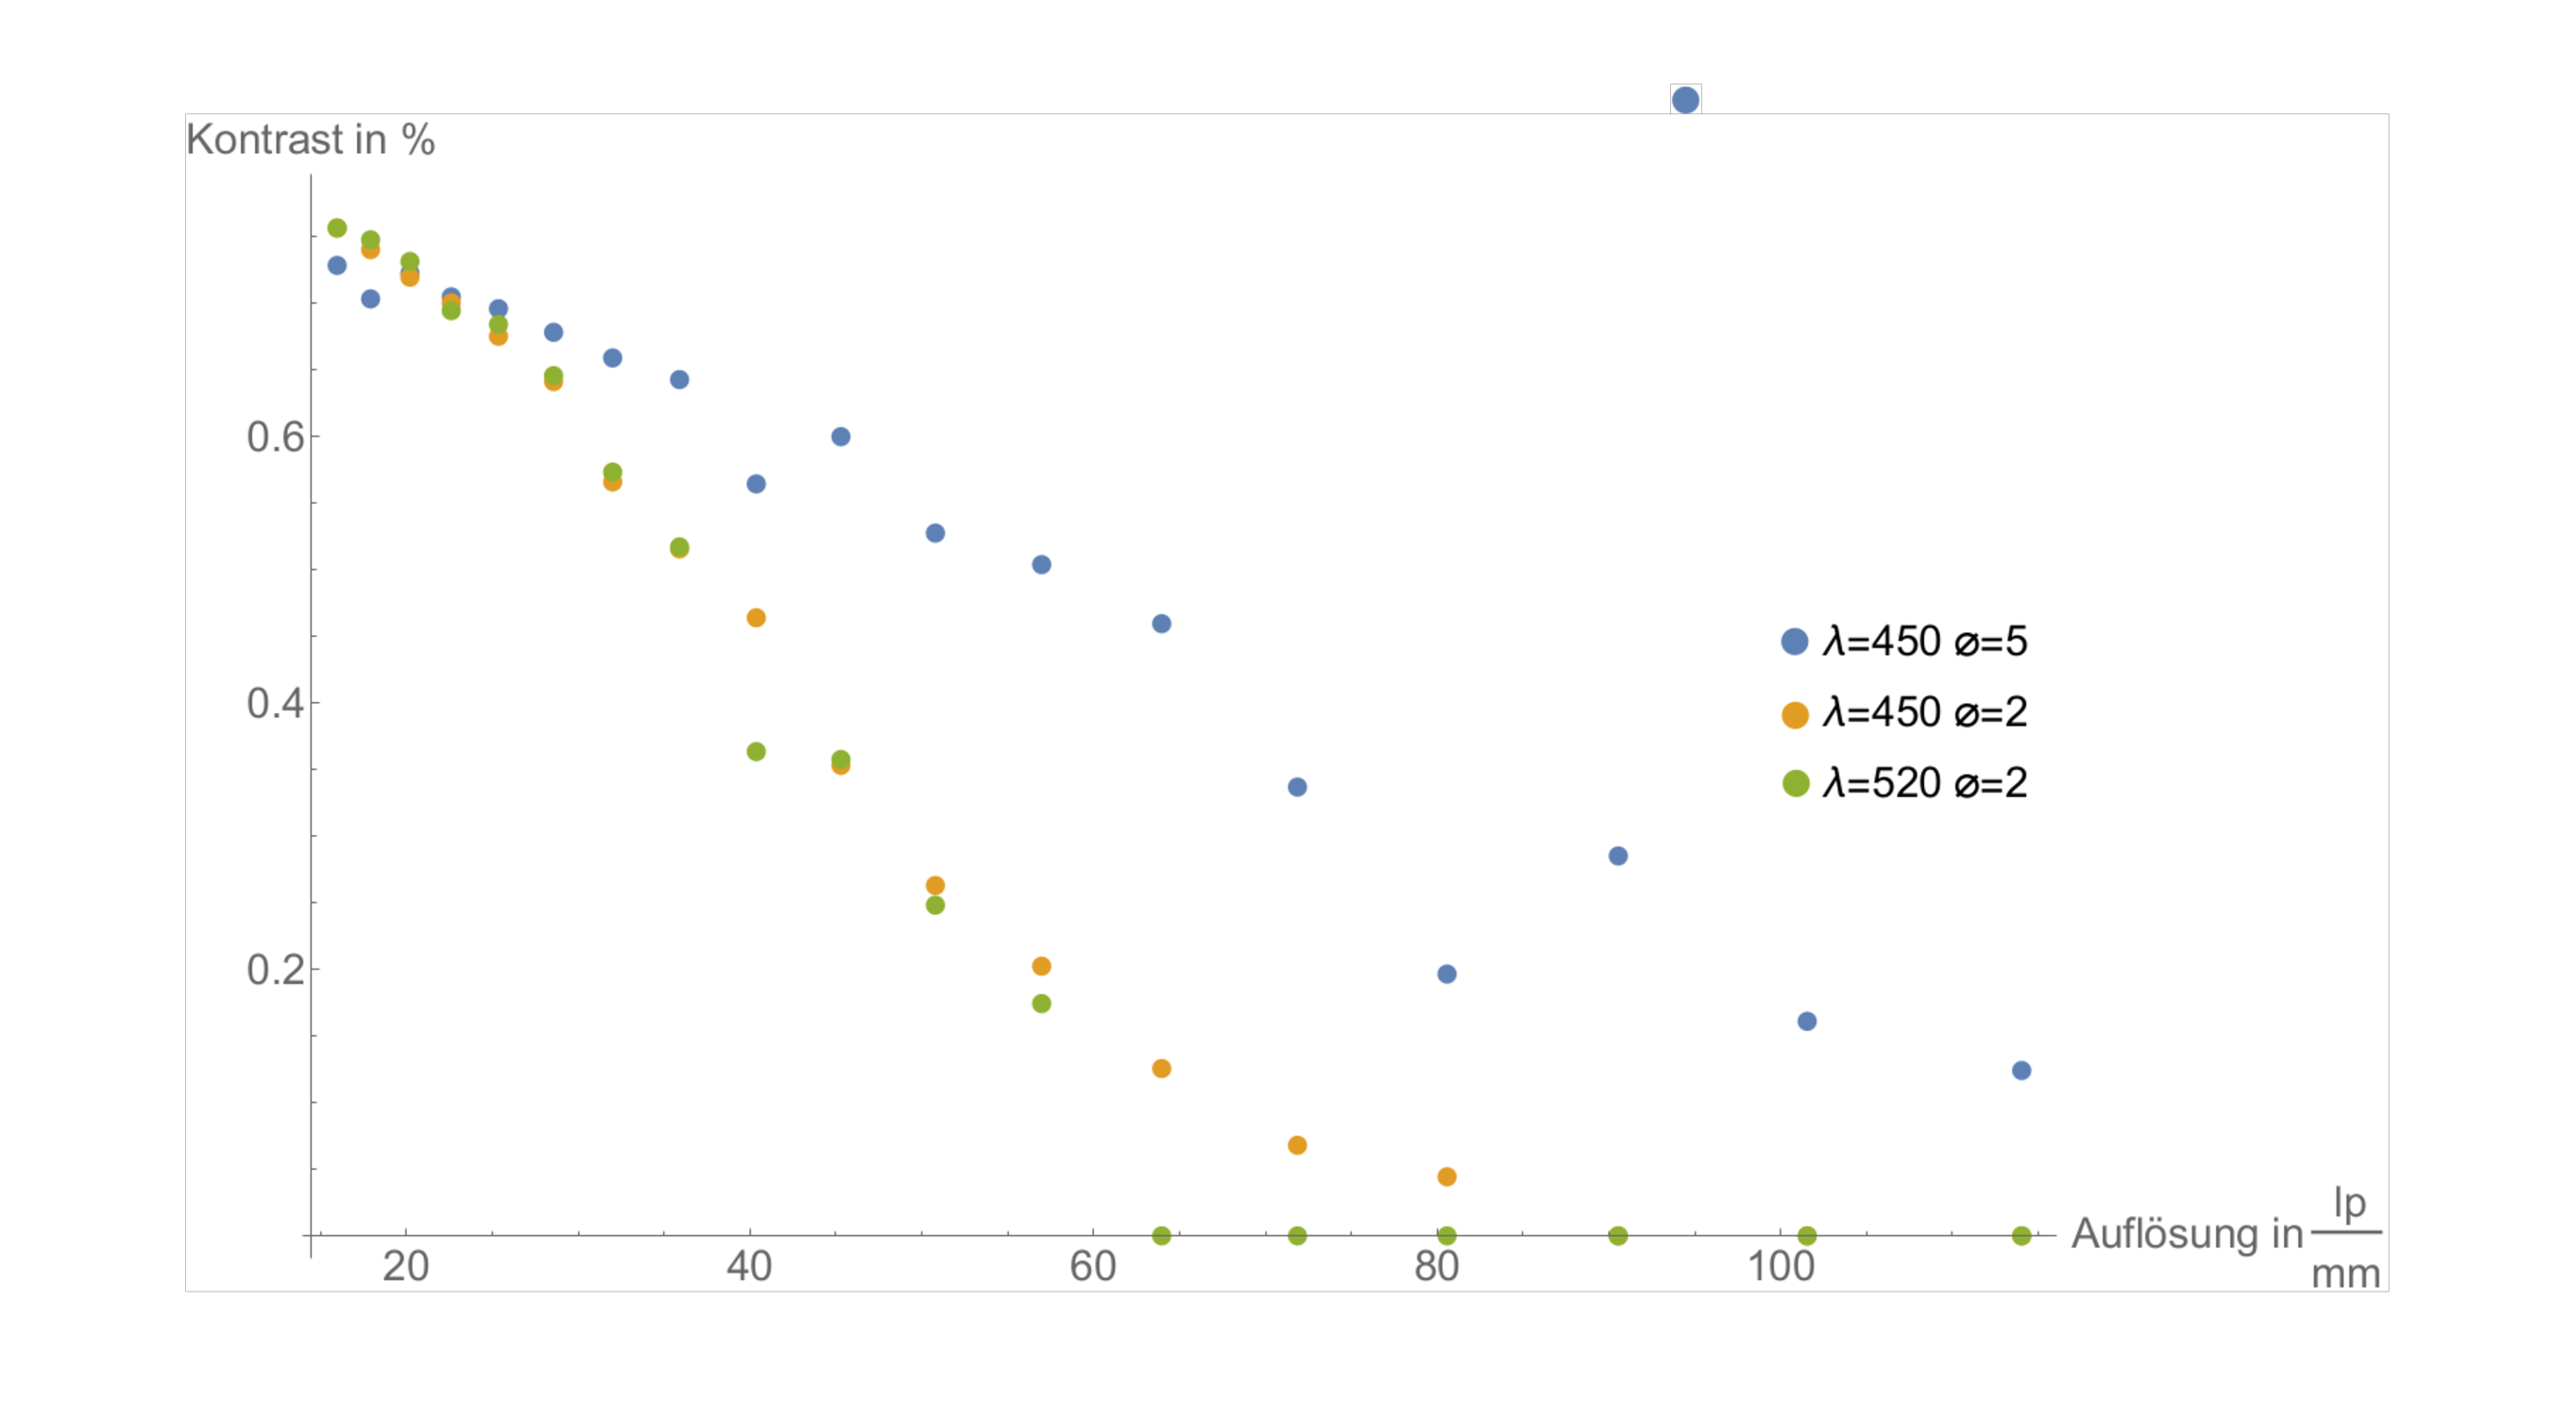
\includegraphics[width=1.0\linewidth]{IMAGE/Versuch2Plot2vertikal2.pdf}
	\caption{Kontrast bei hoher Auflösung (vertikal)}
	\label{fig:Versuch2_Plot2v2}
\end{figure} 
Auch bei hoher Auflösung verbessert ein erhöhter Strahlendurchmesser  den Kontrast. Zwar ist der Kontrast bei einer geringen Auflösung bei einer höheren Wellenlänge höher, aber ab etwa einer Auflösung von $20 \frac{lp}{mm}$ erhöht eine kleine Wellenlänge den Kontrast.

Weiterhin sind die Modulationsübertragungsfunktionen für hohe Auflösungen in Abbildung \ref{fig:Versuch2_Plot2_all} dargestellt, um diese untereinander besser vergleichen zu können.

\begin{figure}[H]
\centering
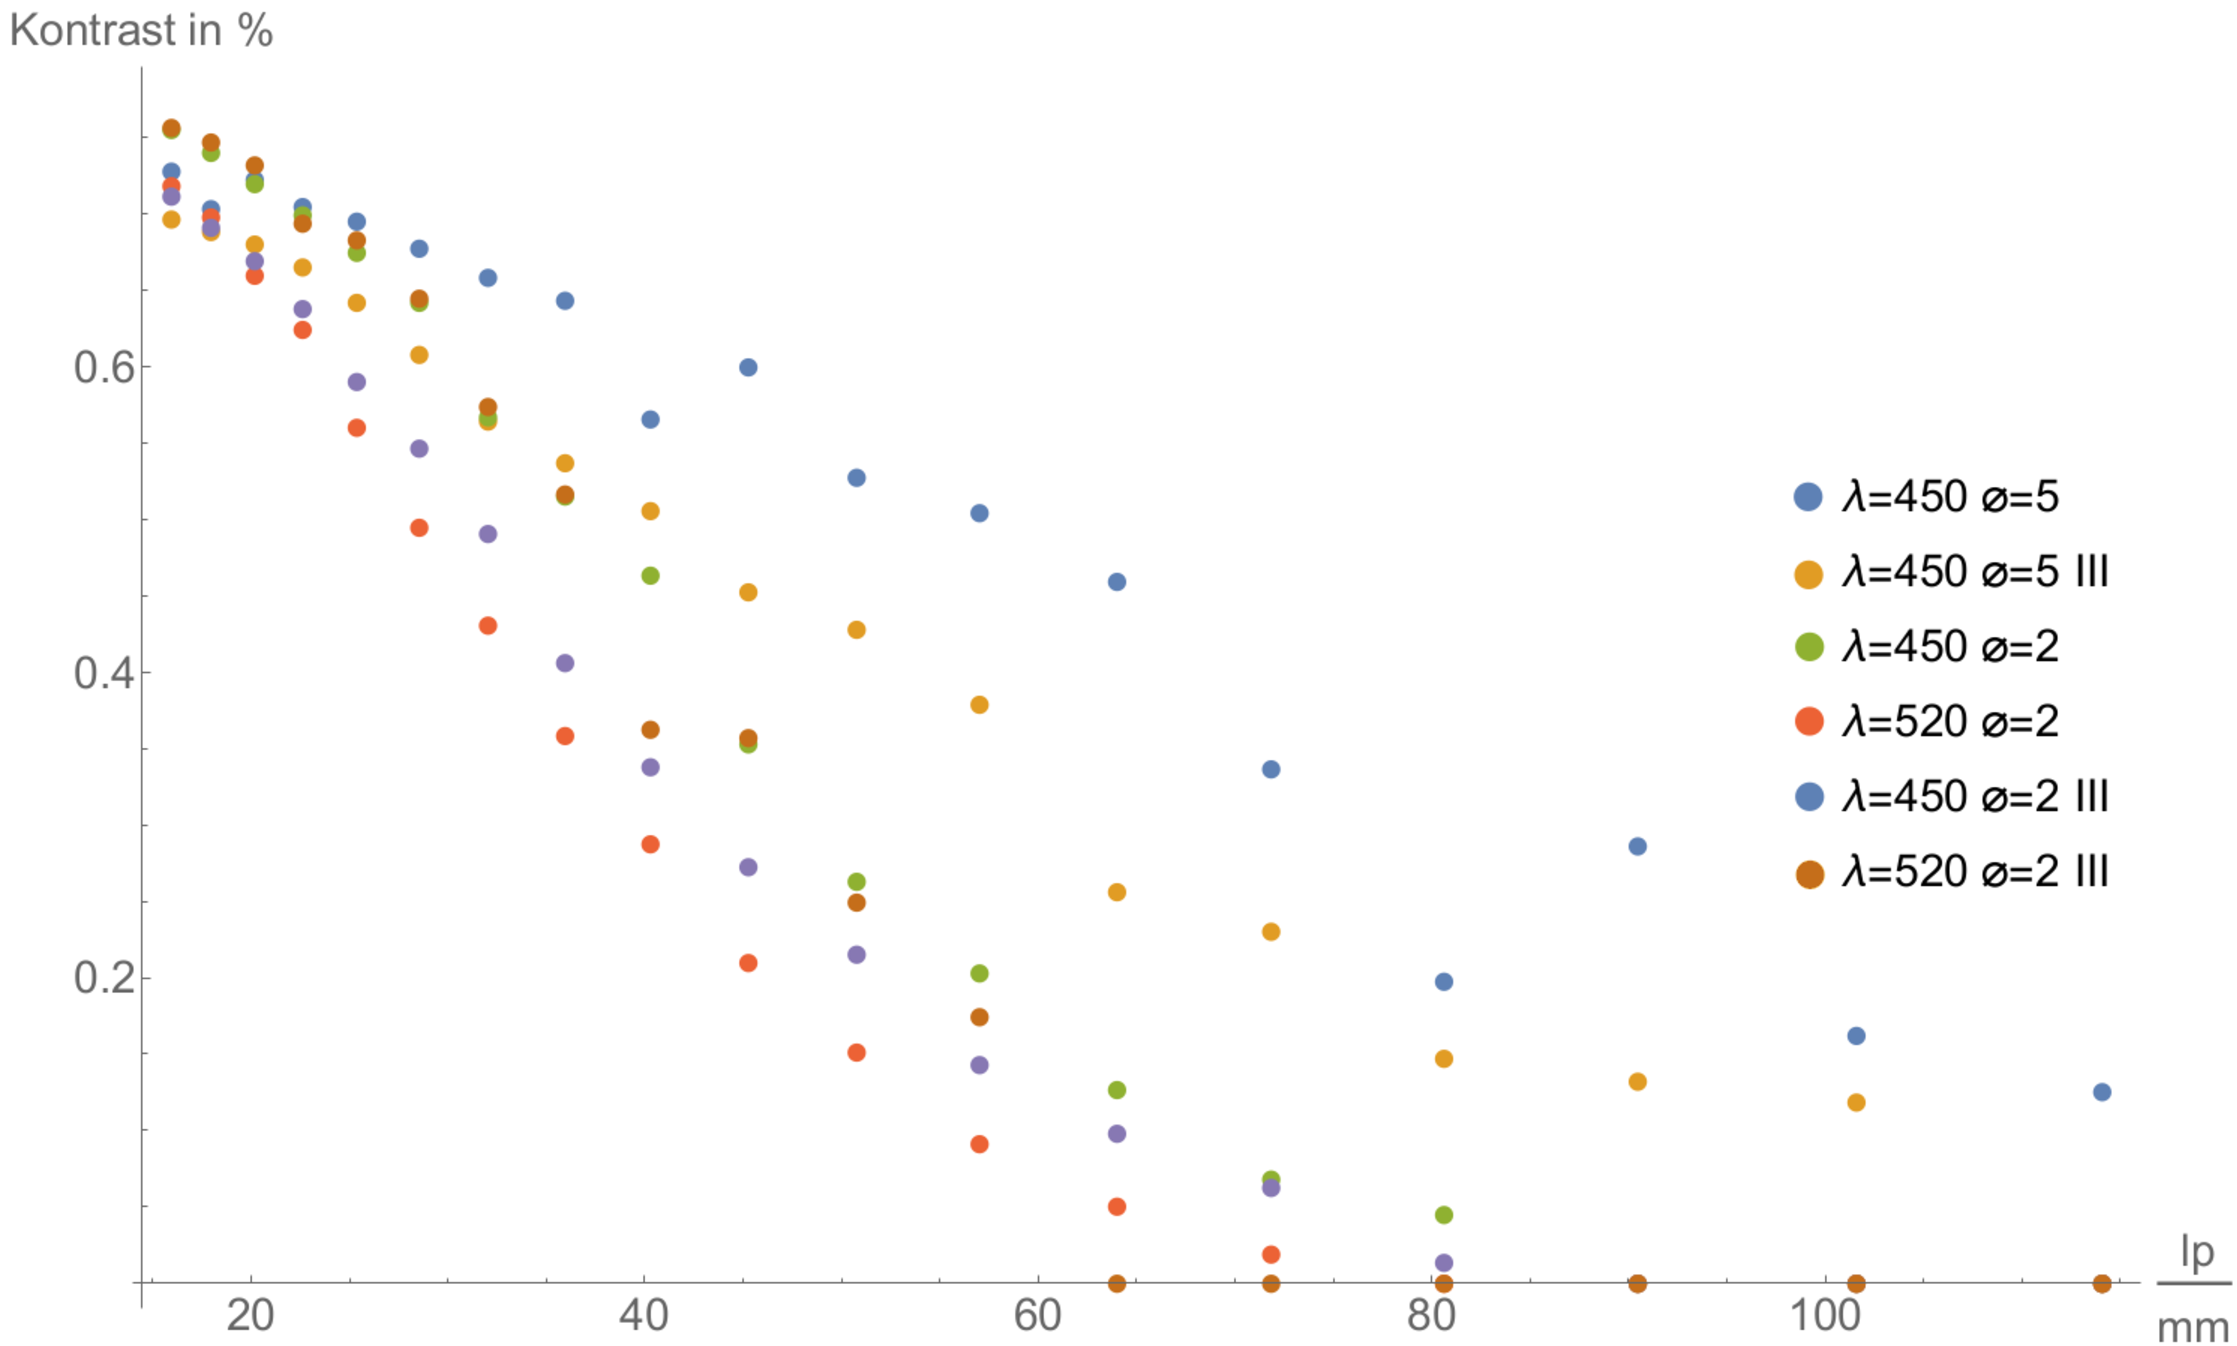
\includegraphics[width=1.0\linewidth]{IMAGE/Versuch2Plot2_all.pdf}
	\caption{Kontrast bei hoher Auflösung (horizontal \& vertikal) \textcolor{red}{Ausführlicher. Wozu vertikal, horizontal Vergleich?}}
	\label{fig:Versuch2_Plot2_all}
\end{figure}

%\textcolor{red}{Vielleicht sollte man die Innere mit der Äußeren Aufnahme zusammensetzen und im selben Plot anzeigen, um längere Messkurven zu erhalten.}


%%%%%%%%%%%%%%%%%%%%%%%Ab hier alte Vorlage%%%%%%%%%%%%%%%%%%%%%%%%%%%%%%%%%%%%
\subsection{Aufnahmen von Heuschreckengehirnen}
In diesem Versuchsabschnitt wurde als Probe ein präpariertes Heuschreckengehirn gewählt.
Die Probe wurde in einer Küvette von oben in Glycerin getaucht und wurde um die $z$-Achse gedreht.
Mit einer 360°-Drehung um die $z$-Achse wurden die Aufnahmen unter verschiedenen Winkeln aufgenommen.
Interessant war bei dieser Messung, dass die Fluoreszenz mit dem Photomultiplier (PMT) darstellt werden konnte, da es sich hier, im Gegensatz zum USAF-Target, um eine dreidimensionale Probe handelt, die fluoresziert.

\subsubsection{Korrektur der Schieflage}
Die durchschnittliche Schieflage der Probe $\alpha$ konnte bei der Auswertung ausgeglichen werden.
Dazu wurde der Drehachsendurchlauf am oberen und unteren Bildrand gemessen und der Winkel $\alpha$ nach folgender Formel berechnet:
$$\alpha = \arcsin \left( \frac{\Delta{x_{\text{oben}}} - \Delta{x_{\text{unten}}}}{y_{\text{max}}} \right) .$$

Hier entspricht $y_\text{max}$ der Anzahl der Pixel auf der $y$-Achse im Bild.
$\Delta{x_\text{oben}}$ und $\Delta{x_\text{unten}}$ beziehen sich hierbei auf die äußersten Pixel am Bildrand oben und unten.

Um $\Delta{x_{\text{oben}}}$ und $\Delta{x_{\text{unten}}}$ zu messen wurde die jeweilige Ebene mit 100 verschiedenen $x$-Achsenverschiebungen mit  \glqq tilt\grqq{} rekonstruiert und anschließend das beste Bild herausgesucht (Reduzierung der Ringartefakte).

Im Folgenden wurde die Aufnahme mit \glqq ImageJ\grqq{} um den jeweiligen Winkel gedreht und das Ergebnis wieder mit  \glqq tilt\grqq{} , aber dieses Mal für alle Ebenen rekonstruiert.
Dabei wurde auch die mittlere $x$-Achsenverschiebung beachtet:
$$\Delta{x} = \frac{\Delta{x_{\text{oben}}} - \Delta{x_{\text{unten}}}}{2}\text{ }.$$

\subsubsection{Darstellung der Rekonstruktion}
Eine Verlängerung der Integrationszeit $\Delta{t}$ von $1$ zu $2$ Sekunden hatte nur eine Aufhellung des PMT-Bildes zur Folge.
Da bei dieser Aufnahme jedoch ein unpassender Filter verwendetet wurde, zeigt das PMT-Bild auch nur das gestreute Licht. Das Ergebnis ist in Abbildung \ref{fig:lang-int} zu sehen.

\begin{figure}[ht]
\centering
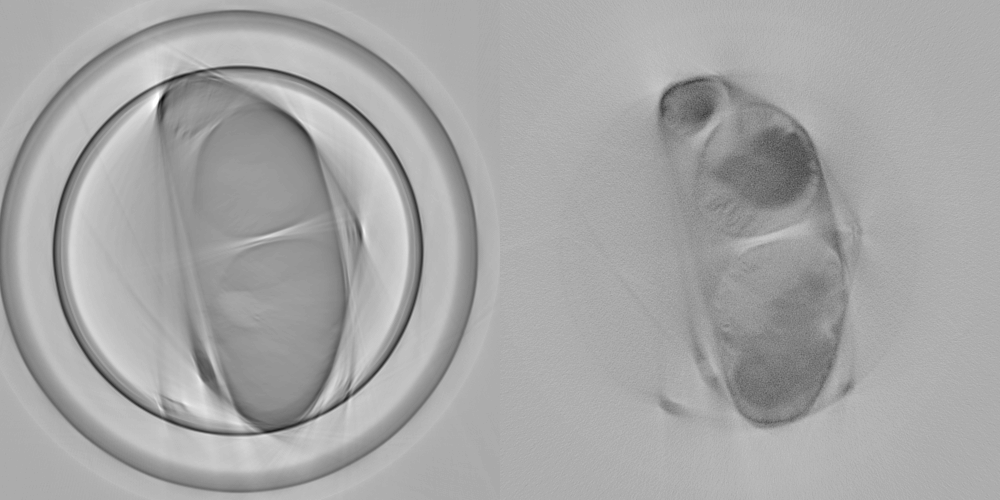
\includegraphics[width=\linewidth]{IMAGE/both-2-450-5-1-c.png}
\caption{Rekonstruktion: Photodiode links, PMT rechts; $\lambda = 450 \text{ } \si{nm}$, $\Delta{t} = 2 \text{ } \si{s}$, $\lambda_\text{Filter} = (520 \pm 36) \text{ } \si{nm}$, $d_\text{Strahl} = 5 \text{ } \si{mm}$, Kontrast angepasst}
	\label{fig:lang-int}
\end{figure}

Mit der Photodiode lassen sich die äußeren Umrisse gut erkennen, mit dem Photomultiplier sogar die Dichte im Inneren.

\begin{minipage}{\linewidth}
In Abbildung \ref{fig:both-pht} sind 2 Rekonstruktionen der Bilder der Photodiode dargestellt.
Es ist erkennbar, dass das Bild mit der längeren Wellenlänge feinere Strukturen im Heuschreckengehirn auflöst.
\begin{figure}[H]
\centering
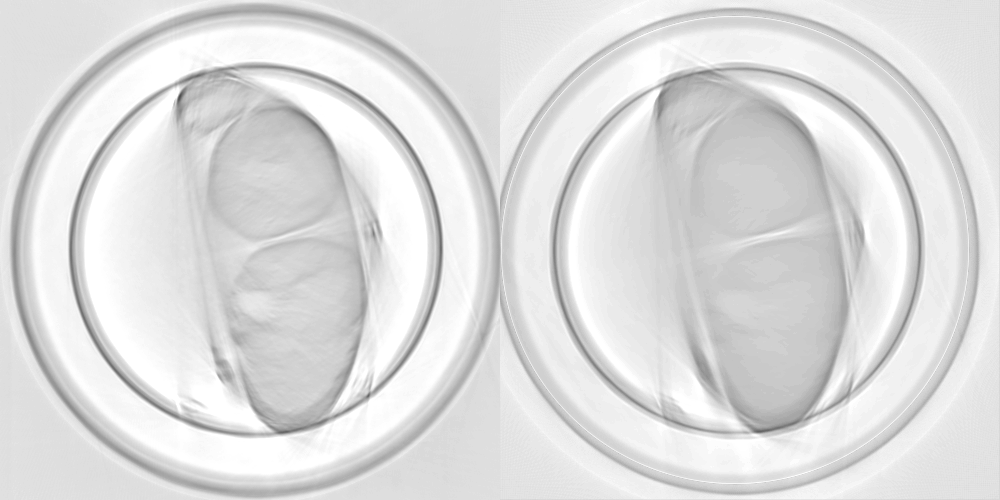
\includegraphics[width=\linewidth]{IMAGE/2-pht-c.png}
\caption{Rekonstruktion: $\lambda = 520 \text{ } \si{nm}$ links, $\lambda = 450 \text{ } \si{nm}$ rechts; Photodiode, $\Delta{t} = 1 \text{ } \si{s}$, $\lambda_\text{Filter} = (520 \pm 36) \text{ } \si{nm}$, $d_\text{Strahl} = 5 \text{ } \si{mm}$, Kontrast angepasst}
	\label{fig:both-pht}
\end{figure}
\end{minipage}

In Abbildung \ref{fig:both-pmt} wurden Bilder des PMT vom jeweiligen Fluoreszenzlicht der Laser rekonstruiert. Im Vergleich ist festzustellen, dass bei $\lambda= 520 \text{ } \si{nm}$ die Auflösung höher ist.

\begin{figure}[H]
\centering
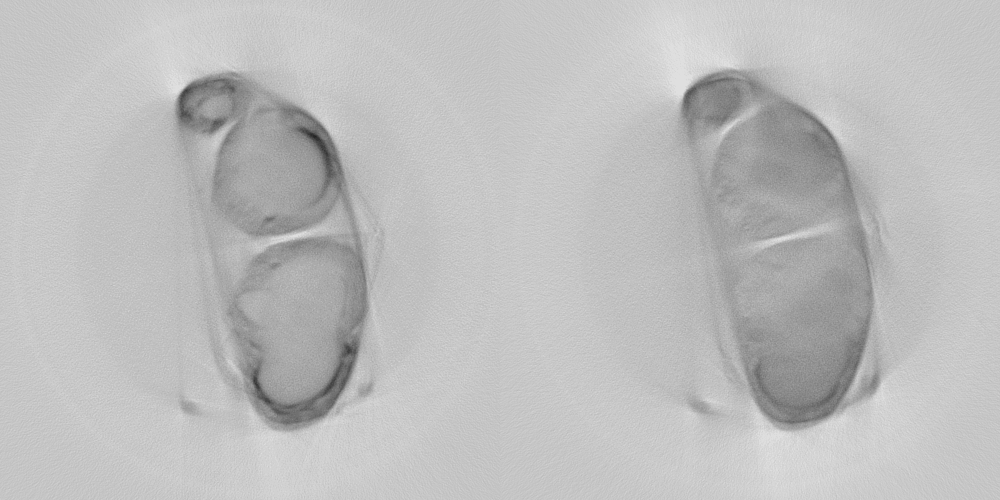
\includegraphics[width=\linewidth]{IMAGE/2-pmt-c.png}
\caption{Rekonstruktion: $\lambda = 520 \text{ } \si{nm}$ mit $\lambda_\text{Filter} = (676 \pm 29) \text{ } \si{nm}$ links,\\
	$\lambda = 450 \text{ } \si{nm}$ mit $\lambda_\text{Filter} \ge 570 \text{ } \si{nm}$ rechts; PMT, $\Delta{t} = 1 \text{ } \si{s}$,\\
$d_\text{Strahl} = 5 \text{ } \si{mm}$, Kontrast angepasst}
	\label{fig:both-pmt}
\end{figure}

Mit dem ImageJ-Plugin \glqq Volume Viewer\grqq{} , ist es nach der Rekonstruktion möglich verschiedene Ansichten auf das Heuschreckengehirn zu generieren. Ein mögliche Ansicht ist in Abbildung \ref{fig:3d} dargestellt.

\begin{figure}[H]
\centering
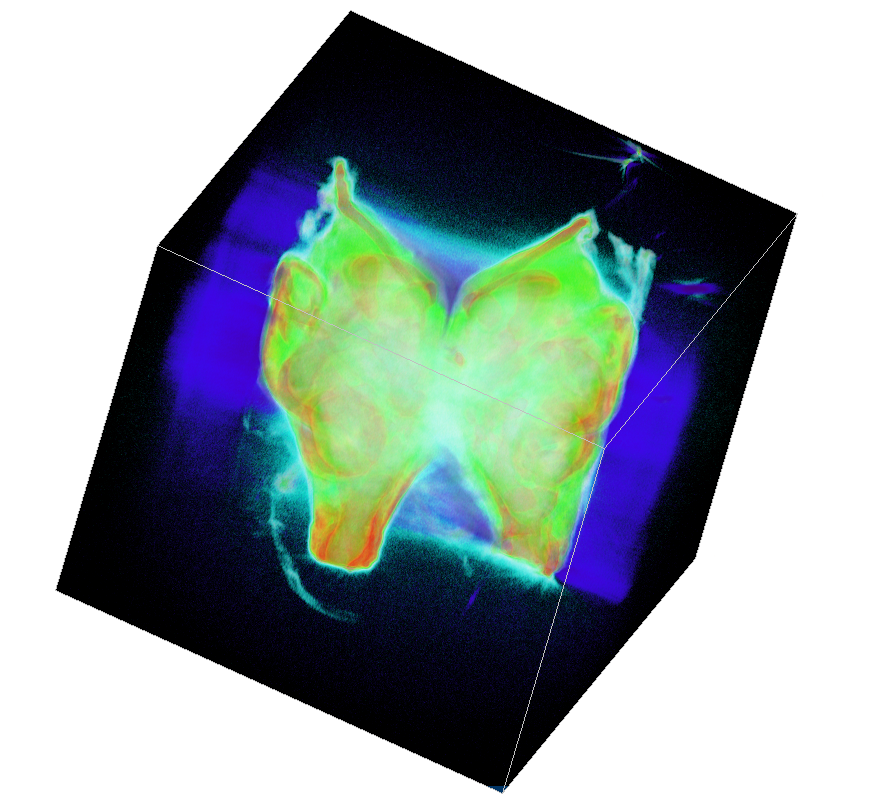
\includegraphics[width=\linewidth]{IMAGE/3dtomo.png}
\caption{3-dimensionale Ansicht einer PMT-Aufnahme: $\lambda = 520 \text{ } \si{nm}$ mit\\ $\lambda_\text{Filter} = (676 \pm 29) \text{ } \si{nm}$, $\Delta{t} = 1 \text{ } \si{s}$, $d_\text{Strahl} = 5 \text{ } \si{mm}$}
	\label{fig:3d}
\end{figure}


\subsubsection{Schwiereigkeiten bei der Versuchsdurchführung}
Zum Einen haben wir zum Einfädeln der Laser in eine Glasfaser das Verfahren Beamwalk benutzt. Da dies aber sehr lange gedauert hat haben wir es darum ergänzt, dass man beim korrigieren der Spiegel immer ein bisschen weiter dreht als das Maximum der Intensität.
Das haben wir gemacht, da der normale Beamwalk das absolute Maximum nur nach unendlich vielen Schritten erreicht.
Wenn man aber die Schritte über das Maximum hinaus macht, dann kommt man schneller zum Maximum, kann es jedoch je nach Schrittgröße nicht erreichen, da man es überspringt.
Ab diesem Punkt führt man wieder den normalen Beamwalk durch.

Man kann unser Verfahren vergleichen mit einer alternierenden Reihe, die schneller konvergiert, als wenn man den Betrag der Reihenglieder betrachten würde.

Eine weitere Schwierigkeit ist bei den Messungen mit sich drehender Probe aufgetreten.
Man musste die Drehachse genau senkrecht positionieren, damit sie nicht präzessiert.
Dies konnten wir durch unsere Justage und die limitierte Genauigkeit der direkten Bildanzeige nicht ganz verhindern.
In der Auswertung konnten wir dann leider auch nur die mittlere Schieflage korrigieren.

In der Theorie sollte jedoch auch eine Korrektur der Präzession nach der Aufnahme noch möglich sein.
Dazu müsste man jedes Bild einer 360°-Aufnahme um den richtigen Betrag drehen, den man mit einem Sinus berechnen könnte, wenn man die maximale Abweichung während der Präzession kennt.

In unserem Fall wanderte die Achse circa 4 Pixel in horizontaler Richtung, was für unser Ergebnis noch in Ordnung war.

\subsubsection{Analyse}
Wie erwartet lassen sich in den Aufnahmen mit dem PMT die inneren Strukturen besser erkennen, da hier die Fluoreszenz aufgenommen wurde.
In Abbildung \ref{fig:both-pmt} kann man außerdem sehen, dass verschiedene Wellenlängen unterschiedliche Bereiche verschieden stark zum Fluoreszieren bringen.

Das unser Meinung nach beste Ergebnis konnten wir beim PMT mit der Kombination des $520\text{ } \si{nm}$-Lasers und dem $(676 \pm 29)\text{ } \si{nm}$-Filter erzeugen.
Deshalb ist dies nochmal mit einer 3-dimensionalen Ansicht des gesamten Heuschreckengehirns abgebildet.

Wir hatten kein Problem mit zu starker Absorption, wie sie nach Lorbeer \cite{slot_paper} bei einer zu großen Probe auftritt.

Insgesamt sind wir mit den Ergebnissen unserer Messung zufrieden.

\section{Diskussion}
\textcolor{red}{Text!}

\section{Fazit}
\textcolor{red}{Text!}

\section{Ausblick}
\textcolor{red}{Text!}

%\listoftables
\clearpage
\listoffigures
%\clearpage
\begin{thebibliography}{99}
%	\bibitem{Schaltung1} \textsc{Saure aus Wikimedia Commons}, \emph{Gleichrichter-Schaltung mit Glättung} (26. August 2009) (Stand: 08.03.2018) \url{https://commons.wikimedia.org/w/index.php?title=File:Gleichrichter-Schaltung.svg&oldid=291347227&uselang=de}
\bibitem{Anleitung} \textsc{Lena Nolte}, \emph{Versuchsanleitung: IQ18 SLOT für das Laborpraktikum Atom- und Molekühlphysik
der Leibniz Universität Hannover} (2015) 

\bibitem{slot_paper} \textsc{Raoul-Amadeus Lorbeer}, \emph{Dreidimensionale und effiziente Erfassung mesoskopischer Proben} (2013) 
\end{thebibliography}



\end{document}
